\documentclass[final,3p,times]{elsarticle}
\usepackage{amsmath,amssymb,amsthm}
\usepackage{graphicx}
\usepackage{booktabs}
\usepackage{array}
\usepackage{microtype}
\usepackage{hyperref}
\hypersetup{hidelinks}
\usepackage{lineno}
\modulolinenumbers[5]
\emergencystretch=1em
\journal{Journal of Computational Physics}
\myfooter[R]{\today}
\newtheorem{proposition}{Proposition}

% New manuscript written from scratch.
% No prose, section structure, or experiment numbering has been copied.
% Compact Elsevier 3p single-column layout; review line numbers retained.
% Editorial plan: REVISION_PLAN.md in this directory.
% Narrative: diagnose deployment failures, evaluate an empirical criterion,
% and assess a Sundman-factored intervention within the tested domain.

\begin{document}
\begin{frontmatter}
\title{Learning Time Transformations for Stiff Hamiltonian Systems:
Deployment Reliability and Applicability Boundaries}
% Author order, affiliations and emails supplied by the authors.
% Shuai Zhu confirmed as corresponding author.
\author[naval]{Jiangshan Wang}
\ead{jswanglab@163.com}
\author[guizhou]{Shuxiang Xu}
\ead{614068193@qq.com}
\author[corex]{Shuai Zhu\corref{corresponding}}
\ead{zhushuaisjtu@gmail.com}
\cortext[corresponding]{Corresponding author.}
\affiliation[naval]{organization={Department of Emergency and Trauma,
The First Affiliated Hospital of Naval Medical University},
city={Shanghai}, country={China}}
\affiliation[guizhou]{organization={College of Mechanical Engineering,
Guizhou University}, city={Guiyang}, country={China}}
\affiliation[corex]{organization={Shanghai Iluvatar CoreX Semiconductor Co., Ltd.},
city={Shanghai}, country={China}}

\begin{abstract}
A learned positive time monitor redistributes resolution in Hamiltonian
integration. Continuous-flow equivalence, however, does not guarantee
completion by a finite implicit solver. We examine this boundary using the
Poincar\'e-Adaptive Symplectic Network (PASNet), which couples a learned
monitor to an extended Hamiltonian and implicit midpoint. The analysis
separates the supplied physical-time vector field from the
monitor-dependent endpoint Jacobian. Using the exact Kepler Hamiltonian,
we evaluate independently trained monitors on a prescribed grid of
non-collisional orbits. Raw-state and invariant-input baselines complete
only part of the grid and fail all highest-eccentricity cases, while
manual $g=r$ completes all controls. A sampled reference-orbit diagnostic
identifies most failures retrospectively. Smaller transformed steps with
a larger step budget recover 59.5\% of failed rollouts with verified
endpoint acceptance, at substantial accuracy and work penalties.
Both tested recipes learning a bounded correction to $g=r$ complete all
evaluations. Accompanying initialisation and training differences leave
the radial factor's isolated causal effect unresolved, and no matched-cost
advantage is established. A learned-Hamiltonian fidelity gate admits no
candidates; modal and Duffing tests provide finite scope checks. For the
tested recipes, the evidence supports embedding known time scales in
learned monitors and assessing completion, state accuracy, invariant
variation and work together with the intended numerical solver.
\end{abstract}

\begin{keyword}
Hamiltonian systems \sep time transformation \sep Sundman monitor
\sep implicit midpoint \sep symplectic integration \sep neural networks
\sep solver reliability
\end{keyword}
\end{frontmatter}
\linenumbers

% Complete working draft; release checks remain in CLAIM_MANIFEST.md.
% Existing artifact identifiers belong in an evidence map, not section titles.

\section{Introduction}
\label{sec:introduction}
Brief intervals of rapid motion and widely separated oscillation
frequencies pose distinct difficulties for Hamiltonian integration.
Resolving these scales while retaining geometric structure is a central
task in computational physics. Symplectic methods provide a discretisation
framework, but geometric structure alone certifies neither trajectory
accuracy nor convergence of an implicit solver~\cite{Hairer2006}.
Eccentric Kepler motion concentrates rapid local dynamics near periapsis;
separated oscillation frequencies pose a different resolution challenge
without approaching a singularity. We examine these time-scale challenges
separately from endpoint-iteration failure, which depends on the monitor,
step and finite solver budget. Such failure alone does not classify the
physical system as stiff.

Classical time transformations introduce a clock $\tau$ and a positive
\emph{monitor} $g$ specifying $dt/d\tau=g$. Sundman's three-body work is a
foundational source for time-based regularisation~\cite{Sundman1913}.
Preto and Tremaine construct adaptive symplectic integrators for separable
Hamiltonians, including a Kepler scheme with physical step proportional to
radius~\cite{Preto1999}. Blanes and Iserles study symplectic integration
after time transformations~\cite{Blanes2012}, and Duruisseaux, Schmitt and
Leok use the Poincar\'e construction in adaptive variational
integration~\cite{Duruisseaux2021}. The nonlinear solve is also part of
the numerical design: Ye et al. combine time transformation with a Broyden
quasi-Newton solve in an adaptive gravitational
integrator~\cite{Ye2025}. Our finite-radius, non-collisional Kepler study
concerns endpoint solving. Its scope differs from extension through
collision, studied by Knauf~\cite{Knauf2025}, and from backward error
analysis with its regularity and step-size assumptions~\cite{Reich1999}.

Structure-preserving learning acts on several distinct objects.
Hamiltonian neural networks learn a scalar whose canonical gradient
defines the vector field~\cite{Greydanus2019}; SympNets learn compositions
of symplectic modules~\cite{Jin2020}; and SympFlow composes parametrised
Hamiltonian flow maps with an associated Hamiltonian
representation~\cite{Canizares2024}. Learning is also coupled to
discretisation. Offen and Ober-Bl\"obaum learn an inverse modified
Hamiltonian for a chosen integrator~\cite{Offen2022}; David and M\'ehats
analyse symplectic training losses and a correction for Hamiltonian
identification from discrete observations~\cite{David2023}. Thapar and
Gupta's ASRNN preprint learns separable kinetic and potential energies
through Verlet recurrence from sparse, irregular
observations~\cite{Thapar2026}. These Hamiltonian-learning approaches
provide context for model--discretisation interaction. Here the supplied
Hamiltonian is held fixed while a separate state-dependent time monitor
is learned.

Temporal adaptation has several forms. SympNets addresses irregular
sampling~\cite{Jin2020}; Janik and Benner's time-adaptive
SympNets~\cite{Janik2025} and H\'enonNets~\cite{Janik2026} take the time
increment as an input. The ATLAS-NN preprint of Mou et al. learns temporal
scaling in a trajectory ansatz and transfers fitted parameters to longer
intervals~\cite{Mou2026}. We learn a state-dependent scalar monitor inside
an extended Hamiltonian and deploy it through an implicit solve; we call
this implementation PASNet. The extended Hamiltonian, midpoint rule and
radial monitor are established ingredients. Our contribution is the
deployment evidence for their implementation with a learned monitor,
without claiming priority for learned temporal adaptation or a new general
symplectic construction.

The numerical question is whether a fitted monitor remains usable by its
solver on the deployment domain under finite iteration and resource
budgets. We address this question with $K=g_\theta(z)(\widehat H(z)+p_0)$
and implicit midpoint. On the exact zero-energy flow, the monitor cancels
from the physical-time vector field $J\nabla\widehat H$. Its derivatives
still enter the endpoint Jacobian at a discrete midpoint, and positivity
and invariant inputs provide no bounds on them. This distinction motivates
evaluating the learned monitor together with the solver that executes it.
The main experiments set $\widehat H=H$ to isolate this combination from
Hamiltonian approximation.

Reference diagnostics and solver interventions probe the Kepler failures;
changes to the training domain and a bounded correction to the classical
radial monitor test possible improvements. Initialisation and training
also change, so the radial-monitor comparison concerns complete recipes.
The contributions are:
\begin{enumerate}
 \item An analytical separation of physical-time model error and
 monitor-dependent endpoint solving, with explicit assumptions for
 continuous-flow equivalence and local fixed-point convergence.
 \item A deployment study linking Kepler completion failures to
 periapsis diagnostics, distinguishing retrospective classification
 from use on new checkpoints and measuring the tested solver interventions.
 \item An evaluation of a Sundman-factored learning recipe against
 training-domain changes, with completion, accuracy and work assessed
 under their respective comparison protocols.
\end{enumerate}
The strongest evidence concerns exact-H, finite-radius Kepler deployment.
Applicability boundaries here describe observed completion and
accuracy--work trade-offs on prescribed deployment grids. Their scope
includes the monitor parameterisation, training recipe, transformed step
and finite solver rules. A separate learned-Hamiltonian gate and modal
and Duffing scope checks assess the reach of that evidence. Universal
scaling laws and practical efficiency advantages would require further
analysis and comparisons.

Section~\ref{sec:formulation} presents the formulation and numerical method.
Section~\ref{sec:analysis} gives the continuous-flow and local solver analysis.
Section~\ref{sec:protocol} describes the experimental design.
Section~\ref{sec:results} reports reliability and accuracy--work results.
Section~\ref{sec:discussion} discusses design implications and limitations.
Section~\ref{sec:conclusions} summarises the findings.
% Targeted comparisons and query coverage: LITERATURE_POSITIONING.md.
% The search supports scoped comparisons, not an exhaustive priority claim.

\section{Problem formulation and numerical construction}
\label{sec:formulation}
\subsection{Hamiltonian dynamics and positive time transformations}
\label{sec:time-transformation}
Let $z=(q,p)\in D\subset\mathbb{R}^{2d}$ denote a canonical phase point,
where $D$ is an open domain on which the Hamiltonian $H$ is smooth. The
physical dynamics are
\begin{equation}
 \frac{dz}{dt}=J\nabla H(z),\qquad
 J=\begin{pmatrix}0&I_d\\-I_d&0\end{pmatrix}.
 \label{eq:physical-dynamics}
\end{equation}
The domain excludes singularities; the Kepler study uses non-collisional
orbits with positive periapsis radius.

A \emph{monitor} is a smooth positive scalar function $g_\theta:D\to(0,\infty)$
that defines the time transformation
\begin{equation}
 \frac{dt}{d\tau}=g_\theta(z).
 \label{eq:time-transformation}
\end{equation}
Here $t$ is physical time, $\tau$ transformed time and $\theta$ the trainable
parameters. A smaller monitor allocates a smaller physical increment per
transformed step. Positivity makes the continuous clock increase.
Integration accuracy and solver convergence require separate assessment.

The supplied Hamiltonian $\widehat H$ is either the exact $H$ or a frozen
learned approximation $H_\psi$. The main experiments fix $\widehat H=H$;
a separate fidelity gate assesses learned candidates.

\subsection{Extended Hamiltonian and implicit midpoint}
\label{sec:midpoint-construction}
Adjoin the canonical pair $(t,p_0)$ and define the autonomous extended
Hamiltonian~\cite{Duruisseaux2021}
\begin{equation}
 K_\theta(z,p_0)=g_\theta(z)\bigl(\widehat H(z)+p_0\bigr).
 \label{eq:extended-hamiltonian}
\end{equation}
Its equations in transformed time are
\begin{align}
 \frac{dz}{d\tau}
 &=g_\theta J\nabla\widehat H
   +(\widehat H+p_0)J\nabla g_\theta,
 \label{eq:extended-state}\\
 \frac{dt}{d\tau}&=g_\theta(z),\qquad
 \frac{dp_0}{d\tau}=0.
 \label{eq:extended-clock}
\end{align}
Initialisation uses $p_0=-\widehat H(z_0)$ and $t_0=0$. Conservation of
$K_\theta=0$ and positivity give $\widehat H+p_0=0$ along the exact flow
(Section~\ref{sec:analysis}).

The product $K_\theta$ is generally nonseparable even when $\widehat H$
is separable. Implicit midpoint gives a second-order symplectic
discretisation without a kinetic--potential splitting. Other methods
are available: Tao's explicit extended-phase-space construction handles
nonseparability without an implicit solve~\cite{Tao2016}. Here we fix
midpoint to examine how the learned monitor interacts with one specified
endpoint solver.
For a prescribed transformed-time step $h_n>0$, write
$\bar z_n=(z_n+z_{n+1})/2$ and
$F_\theta(z;p_0)=J\nabla_z K_\theta(z,p_0)$. Implicit midpoint gives
\begin{align}
 z_{n+1}&=z_n+h_n F_\theta(\bar z_n;p_0),
 \label{eq:midpoint-state}\\
 t_{n+1}&=t_n+h_n g_\theta(\bar z_n),\qquad p_{0,n+1}=p_{0,n}.
 \label{eq:midpoint-clock}
\end{align}
The clock update approximates
$\Delta t=\int_{\tau_n}^{\tau_{n+1}}g_\theta(z(\tau))\,d\tau$.
The state update differentiates the full product in
\eqref{eq:extended-hamiltonian}: the $\nabla g_\theta$ term cannot be
dropped because a discrete midpoint can lie off the zero-energy surface.

For fixed $z_n$, $p_0$ and $h_n$, the defining endpoint residual is
\begin{equation}
 R_n(y)=y-z_n-h_n F_\theta\!\left(\frac{z_n+y}{2};p_0\right).
 \label{eq:endpoint-residual}
\end{equation}
The fixed-point solver starts from the explicit predictor
\begin{equation}
 y^{(0)}=z_n+h_n F_\theta(z_n;p_0),
 \label{eq:explicit-predictor}
\end{equation}
and iterates
\begin{equation}
 y^{(k+1)}=z_n+h_n F_\theta\!\left(\frac{z_n+y^{(k)}}{2};p_0\right).
 \label{eq:fixed-point-iteration}
\end{equation}
Newton-based controls instead solve the endpoint equation using its
Jacobian, with the damping and stopping rules specified by the respective
evaluation protocol.

Endpoint acceptance distinguishes
$u_k=\|y^{(k+1)}-y^{(k)}\|_\infty$ and
$r_k=\|R_n(y^{(k+1)})\|_\infty$. The fixed-point update equals, up to sign, the residual
at the previous iterate. Verification of the returned endpoint is a
separate check. The original runs stopped on $u_k$; the verification
study also checks the returned residual (Section~\ref{sec:protocol}).

The exactly solved midpoint map is symplectic in the extended canonical
variables when the step size is prescribed independently of the
state~\cite{Hairer2006}.
It implies neither exact conservation of non-quadratic $K_\theta$ nor
exact symplecticity of finite iterations.
For comparisons at a common physical horizon $T$, an overshooting step is
replaced by a shorter transformed-time step. In the main deployment runner,
this step is found by bisection, repeatedly solving the endpoint equation
and comparing $h_n g_\theta(\bar z_n)$ with $T-t_n$. After the finite search,
the recorded clock is set to $T$, whereas the state is the last computed
candidate. The final step depends on the current state, so symplecticity of the entire
horizon-matched map does not follow from the fixed-step property.

\subsection{Monitor parameterisations and training}
\label{sec:monitor-training}
The main planar Kepler studies use dimensionless variables and
$H(q,p)=\|p\|^2/2-1/r$, with $r=\|q\|>0$. Let $f_\theta$ be a scalar
multilayer perceptron with two hidden layers of width 64 and hyperbolic
tangent activations, and let $\sigma(s)=(1+e^{-s})^{-1}$.
The complete extended-phase-space implementation, including these monitor
parameterisations and the implicit-midpoint rollout, is referred to as
PASNet in what follows.\footnote{Here PASNet abbreviates
Poincar\'e-Adaptive Symplectic Network. It is distinct from the
Physics-informed Adaptive Scale Deep Operator Network named PAS-Net
by Mou et al.~\cite{Mou2025PAS}, which uses coordinate-scale embeddings
for PDE operator learning.}
We compare
\begin{align}
 g_\theta^{\mathrm{raw}}(z)&=2\sigma\bigl(f_\theta(z)\bigr),
 \label{eq:raw-monitor}\\
 g_\theta^{\mathrm{inv}}(z)&=2\sigma\bigl(f_\theta(\phi(z))\bigr),
 \label{eq:invariant-monitor}
\end{align}
where the invariant input is
\begin{equation}
 \phi(z)=\bigl(r,r^{-1},\|p\|^2,(q\cdot p)^2,L^2\bigr),
 \qquad L=q_1p_2-q_2p_1.
 \label{eq:invariant-features}
\end{equation}
These features are unchanged by simultaneous planar rotations of $q$ and
$p$, and by momentum reversal $p\mapsto-p$. The raw monitor imposes neither
property. Both outputs lie in $(0,2)$ in exact arithmetic, which bounds
their discrete physical-time increment by $2h_n$.

The structural intervention retains the invariant input and factors out
the classical Kepler monitor:
\begin{equation}
 g_\theta^{\mathrm{fact}}(z)=r\,c_\theta(z),\qquad
 c_\theta(z)=2\sigma\bigl(f_\theta(\phi(z))\bigr).
 \label{eq:factored-monitor}
\end{equation}
Consequently $0<g_\theta^{\mathrm{fact}}<2r$, and the monitor vanishes as
$r\to0$ along non-collisional states approaching the singular set.
The global cap of 2 on the unfactored monitors is replaced by a cap on the
multiplicative correction; $g_\theta^{\mathrm{fact}}$ need not be below 2
when $r>1$. The value bound constrains neither derivatives nor endpoint convergence.

The principal checkpoints are trained independently through numerical
rollouts with $\widehat H=H$. For a rollout containing $N$ steps, put
$E_n=\widehat H(z_n)$ and $\bar E=(N+1)^{-1}\sum_{n=0}^N E_n$. The
implemented objective is
\begin{align}
 \mathcal L(\theta)
 &=w_E\mathcal V_E+w_z\mathcal L_z+\lambda_g\mathcal C_g,
 \label{eq:monitor-loss}\\
 \mathcal V_E&=\frac1N\sum_{n=0}^N(E_n-\bar E)^2,\qquad
 \mathcal C_g=\frac1{N+1}\sum_{n=0}^N\frac1{g_\theta(z_n)},
 \label{eq:energy-cost-loss}\\
 \mathcal L_z&=\frac1{2dM}\sum_{j=1}^M
   \|\widetilde z(s_j)-z_{\mathrm{ref}}(s_j)\|_2^2.
 \label{eq:checkpoint-loss}
\end{align}
Here $s_j$ are relative physical checkpoint times, $z_{\mathrm{ref}}$ the
exact Kepler solution, and $\widetilde z(s_j)$ the linear interpolation
between bracketing numerical states. The energy term is discrete sample
variance; the inverse-monitor term discourages small increments but is
not measured solver work.

Training uses 100 steps at $h=0.08$, with four fixed-point updates after
each explicit predictor, and weights $(w_E,w_z,\lambda_g)=(0.1,5,0.02)$.
Gradients pass through endpoint states only: clock interpolation weights
and checkpoint selection are detached. The finite unrolling therefore
differs from deployment at a solver tolerance. Checkpoint selection
minimises validation state MSE on the training orbit. Supplementary
Material, Section S2.3, gives the optimisation, sampling and validation
details.

Unfactored and factored final-layer biases are $-2.2$ and 0, respectively,
with random weights of standard deviation 0.1. The factored monitor is
therefore not initialised identically to $g=r$. The recipe comparison includes this difference,
so it does not isolate the factor $r$.

A separate architecture--solver control fits raw and invariant students
to the outputs of a single frozen teacher monitor using supervised
mean-squared error. These distilled students are distinguished from
independently rollout-trained checkpoints throughout the results; multiple
student seeds do not constitute independent teacher training runs.

Symbols are defined at first use; Supplementary Material, Table S1,
collects the notation for reference.

\section{Continuous-flow equivalence and local solver analysis}
\label{sec:analysis}

The analysis proceeds from the exact transformed flow to a single
midpoint endpoint equation and then to a sampled reference diagnostic.
The endpoint and reference arguments remain local or sampled; neither
establishes global discrete convergence.

\subsection{Physical-time equivalence and Hamiltonian error}
\label{sec:continuous-equivalence}

\begin{proposition}[Zero-energy flow equivalence]
\label{prop:flow-equivalence}
Let $\widehat H,g_\theta\in C^1(D)$, let $g_\theta>0$ along a classical
solution of \eqref{eq:extended-state}--\eqref{eq:extended-clock}, and set
$p_0=-\widehat H(z_0)$. If the solution remains in $D$, then
$\widehat H(z(\tau))+p_0=0$ for every point on that solution. Wherever
$dt/d\tau$ is used as a clock, the physical-time trajectory satisfies
\begin{equation}
 \frac{dz}{dt}=J\nabla \widehat H(z).
 \label{eq:physical-equivalence}
\end{equation}
Thus a positive monitor changes the parameterisation of the supplied
Hamiltonian flow; it does not change that vector field in physical time.
\end{proposition}

\begin{proof}
The extended Hamiltonian is conserved by its exact canonical flow. Its
initial value is $K_\theta(z_0,p_0)=0$. Since $g_\theta>0$, conservation of
$K_\theta=g_\theta(\widehat H+p_0)$ implies
$\widehat H+p_0=0$. The second term in \eqref{eq:extended-state} therefore
vanishes, leaving $dz/d\tau=g_\theta J\nabla\widehat H$. Dividing by
$dt/d\tau=g_\theta$ gives \eqref{eq:physical-equivalence}.
\end{proof}

This identity for the exact flow does not ensure that finite midpoint
solves remain on the zero-energy surface. To quantify the effect of using $\widehat H\ne H$, suppose that $H,\widehat H\in
C^1(D)$ and that the physical trajectory remains in a compact set
$\Omega\Subset D$ for $0\le t\le T$. Define
\begin{equation}
 \epsilon_H=\sup_{z\in\Omega}
       \left\|\nabla\widehat H(z)-\nabla H(z)\right\|_2,
 \qquad
 C_H=\sup_{z\in\Omega}\|\nabla H(z)\|_2.
 \label{eq:hamiltonian-gradient-error}
\end{equation}
Along the physical-time flow in \eqref{eq:physical-equivalence},
\begin{align}
 \frac{d}{dt}H(z(t))
 &=\nabla H(z)^{\mathsf T}J\nabla\widehat H(z)\\
 &=\nabla H(z)^{\mathsf T}J
       \bigl(\nabla\widehat H(z)-\nabla H(z)\bigr),
 \label{eq:true-energy-derivative}
\end{align}
because $v^{\mathsf T}Jv=0$ for every vector $v$. Since the canonical
matrix $J$ is orthogonal in the Euclidean norm,
\begin{equation}
 \left|H(z(T))-H(z(0))\right|
 \le C_H\,\epsilon_H\,T.
 \label{eq:true-energy-upper-bound}
\end{equation}
The monitor cancels from both the physical-time vector field and the bound.
Equation~\eqref{eq:true-energy-upper-bound} is an upper bound on energy
variation. It provides no nonzero lower bound and no bound on state,
phase or discrete error. An incorrect Hamiltonian can still preserve
true energy in special cases. When $\widehat H=H$, only discretisation
and finite endpoint solving introduce energy error.

For the Kepler system, $D$ excludes $q=0$ and the compact set must have a
positive minimum radius. The estimate therefore does not justify taking a
collision limit or treating a learned-Hamiltonian fidelity test as optional.
The learned-Hamiltonian entry study and its scope are reported separately in
Section~\ref{sec:protocol} and the results section.

% TODO(author): B4. A broader learned-Hamiltonian claim requires at least one
% candidate that passes the fidelity gate; otherwise retain the exact-H scope.

\subsection{Endpoint Jacobian and local fixed-point convergence}
\label{sec:endpoint-analysis}

Assume $\widehat H,g_\theta\in C^2(D)$ and fix $z$, $p_0$, and a
transformed-time step $h>0$. The fixed-point map
associated with \eqref{eq:midpoint-state} is
\begin{equation}
 \Phi_{z,h}(y)=z+hJ\nabla_zK_\theta\!\left(\frac{z+y}{2},p_0\right).
 \label{eq:fixed-point-map}
\end{equation}
Writing $R(y)=y-\Phi_{z,h}(y)$ for the endpoint residual, its derivative is
\begin{equation}
 D_yR(y)=I-\frac{h}{2}J D^2_{zz}K_\theta
              \!\left(\frac{z+y}{2},p_0\right).
 \label{eq:residual-jacobian}
\end{equation}
For $K_\theta=g_\theta(\widehat H+p_0)$, the Hessian entering this expression
is
\begin{align}
 D^2_{zz}K_\theta
 &=g_\theta D^2\widehat H
   +\nabla g_\theta\otimes\nabla\widehat H
   +\nabla\widehat H\otimes\nabla g_\theta
   +(\widehat H+p_0)D^2g_\theta .
 \label{eq:extended-hessian}
\end{align}
All quantities in \eqref{eq:extended-hessian} are evaluated at the same
midpoint. The last term vanishes on the exact zero-energy surface, but a
finite midpoint iterate need not lie on that surface. The monitor therefore
affects the endpoint Jacobian both through its value and through its first
and second derivatives.

An operator-norm condition gives a conventional local sufficient criterion.
Let $V$ be a nonempty closed convex subset of the finite-dimensional
endpoint space. Thus $V$ is complete under the chosen vector norm. Assume
$\Phi_{z,h}(V)\subseteq V$, and that the midpoint set
$M=\{(z+y)/2:y\in V\}$ lies in the differentiability domain. Suppose that
\begin{equation}
 \kappa_V=\frac{h}{2}\sup_{w\in M}
       \left\|J D^2_{zz}K_\theta(w,p_0)\right\|<1,
 \label{eq:banach-sufficient-condition}
\end{equation}
where the matrix norm is induced by the same vector norm. Convexity allows
the derivative bound to be integrated along each segment between two
endpoints, so $\Phi_{z,h}$ is a contraction on $V$. Banach's fixed-point theorem
gives a unique fixed point in $V$ together with convergence of the iteration
from every initial endpoint in $V$. A pointwise bound on an arbitrary closed set is insufficient: the self-map,
convexity and completeness assumptions are essential.
Condition~\eqref{eq:banach-sufficient-condition} is local and sufficient.

At an actual fixed point $y_*$, the linearised iteration matrix is
\begin{equation}
 A_* = D_y\Phi_{z,h}(y_*)
     =\frac{h}{2}J D^2_{zz}K_\theta
       \!\left(\frac{z+y_*}{2},p_0\right).
 \label{eq:fixed-point-linearisation}
\end{equation}
If $\rho(A_*)<1$, the fixed point is locally asymptotically attracting for
the differentiable iteration. The operator norm in
\eqref{eq:banach-sufficient-condition} can be larger than $\rho(A_*)$,
especially when $A_*$ is non-normal; conversely, a spectral-radius value
computed at one point says nothing about a different endpoint or about a
global basin of attraction. These distinctions motivate the empirical
reference-orbit statistic below. They leave global discrete stability
unresolved.

% TODO(author): B6. A discrete proposition would need explicit invariant
% domains, step-size restrictions, regularity, and solver acceptance rules.

\subsection{Reference-orbit diagnostics and their limits}
\label{sec:reference-diagnostic}

For a prescribed reference state $z_{\mathrm{ref}}$ and a monitor $g_\theta$,
we evaluate the matrix in \eqref{eq:fixed-point-linearisation} at the
reference state, using $\widehat H=H$, $p_0=-H(z_{\mathrm{ref}}(0))$,
and a specified $h$:
\begin{equation}
 A_{\mathrm{ref}}(z_{\mathrm{ref}};h)
 =\frac{h}{2}J D^2_{zz}K_\theta(z_{\mathrm{ref}},p_0),
 \qquad
 \rho_{\mathrm{ref}}(z_{\mathrm{ref}};h)
 =\rho\bigl(A_{\mathrm{ref}}(z_{\mathrm{ref}};h)\bigr).
 \label{eq:reference-rho}
\end{equation}
The orbit statistic used in the diagnostic study is
\begin{equation}
 \rho_{\max}^{\mathrm{ref}}(\mathcal O;h)
 =\max_{z\in\mathcal S(\mathcal O)}
       \rho_{\mathrm{ref}}(z;h),
 \label{eq:reference-rho-max}
\end{equation}
where $\mathcal S(\mathcal O)$ is a finite set of analytically generated
Kepler states sampled uniformly in eccentric anomaly. The implementation
uses 720 samples per reference orbit, float64 automatic-differentiation
Hessians, and the deployment step $h=0.04$. A companion spectral norm is
recorded to compare eigenvalue magnitudes with the Euclidean operator norm.
Its sampled values do not verify a uniform bound on an endpoint self-map
domain as required by \eqref{eq:banach-sufficient-condition}, and it is not
substituted for the spectral radius in the registered classification rule.

The registered empirical rule predicts solver failure when
$\rho_{\max}^{\mathrm{ref}}\ge1$ and completion otherwise. For a fixed
monitor and reference sample set, $A_{\mathrm{ref}}$ scales linearly with
$h$, so $\rho_{\max}^{\mathrm{ref}}(\mathcal O;\alpha h)
=\alpha\rho_{\max}^{\mathrm{ref}}(\mathcal O;h)$ for $\alpha>0$.
This identity motivates the tested step-size intervention
\begin{equation}
 h_{\mathrm{test}}=h\min\!\left(1,
          \frac{0.5}{\rho_{\max}^{\mathrm{ref}}(\mathcal O;h)}\right),
 \label{eq:diagnostic-step-intervention}
\end{equation}
with no change when the statistic is zero. The protocol chooses 0.5;
it has no proof as a safety factor. Rescaling the sampled statistic
certifies neither convergence at the new numerical midpoints nor
accuracy after completion. Section~\ref{sec:results} reports the
intervention outcomes.

The baseline comparison uses known labels; new checkpoints are tested
prospectively (Section~\ref{sec:estimands}). The diagnostic requires a
reference orbit and has not been validated online. Sampling can miss
peaks, numerical midpoints can depart from the reference, and the spectral
radius controls neither non-normal transients nor the nonlinear basin.
Neither threshold outcome is certified.

% TODO(author): B5. Evaluation of the same diagnostic on accepted discrete
% trajectories remains untested and should not be implied by this definition.

\section{Experimental design and validation}
\label{sec:protocol}

The principal comparisons fix $\widehat H=H$ to isolate monitor--solver
effects. Table~\ref{tab:evidence-scope} summarises their scope; supplementary
protocols give configuration, seed and artifact identifiers.

\begin{table}[t]
\centering
\begingroup
\renewcommand{\baselinestretch}{1}
\small
\caption{Experimental evidence and the scope of the corresponding comparisons.
Counts describe evaluation grids, not independent population samples.}
\label{tab:evidence-scope}
\begin{tabular}{@{}>{\raggedright\arraybackslash}p{0.20\textwidth}
>{\raggedright\arraybackslash}p{0.36\textwidth}
>{\raggedright\arraybackslash}p{0.34\textwidth}@{}}
\toprule
Study & Design & Scope \\
\midrule
Deployment reliability & Two architectures, five checkpoints each;
72 scenarios per checkpoint & Exact Kepler $H$; one training orbit \\
Architecture and solver & One teacher; five students per architecture;
two solvers & Distillation; three-period horizon \\
Early conditioning & 1056 recorded rollouts; one accepted-iterate
observation per run at each matched step & Descriptive association;
shared checkpoints and distinct solver protocols \\
Diagnostic and step intervention & 396 reference records; intervention
on 252 failed rollouts & Known baseline labels; conditional intervention \\
Training domain and factorisation & Three arms, five checkpoints each;
1080 evaluations & Prospective diagnostics; recipe differences \\
Accuracy and cost & 38 configurations, 18 scenarios each & Unfactored
monitors; complete-grid front eligibility \\
Cross-system scope & Modal and Duffing; 288 evaluations & Exact $H$;
at most 32 state variables \\
Hamiltonian fidelity & Five candidates; held-out gradient targets &
Entry gate for a learned-$H$ comparison \\
\bottomrule
\end{tabular}
\endgroup
\end{table}

\subsection{Benchmarks, training domains, and evaluation grids}
\label{sec:benchmark-design}
For Kepler, an orbit with semi-major axis $a$ and eccentricity $e$ has
energy $-1/(2a)$, periapsis radius $r_{\mathrm p}=a(1-e)$ and period
$P(a)=2\pi a^{3/2}$. Increasing eccentricity contracts the radius and
local dynamical time scale near periapsis. This event-dependent scale is
distinct from a fixed ratio of oscillatory frequencies in a modal system.
The baseline rollout-training orbit has $a=1$, $e=0.9$, one orientation,
and forward momentum. Five checkpoints are trained for each of the raw
and invariant architectures using separate initialisation seeds and
matched sampling and validation seed streams.

Each checkpoint is evaluated on the Cartesian product
\begin{equation}
\begin{aligned}
 a&\in\{0.75,1,1.25\}, & e&\in\{0.7,0.9,0.99\},\\
 M_0&\in\{\pi,\pi/2\}, & \alpha&\in\{0,\pi/2\},\\
 \eta&\in\{+1,-1\},
\end{aligned}
\label{eq:kepler-deployment-grid}
\end{equation}
where $M_0$ is initial mean anomaly, $\alpha$ is the common rotation of
position and momentum, and $\eta$ specifies momentum direction. The
72 scenarios test a combination of energy-shell, eccentricity and symmetry
changes, as well as cases on the training orbit. They are not all unseen
orbits in the same sense. All runs have physical horizon $T=P(a)$, use
$h=0.04$, and retain the original fixed-point stopping rule with tolerance
$10^{-12}$, at most 100 updates per endpoint and a cap of $10^5$ accepted
steps. The manual $g=r$ control uses the same grid and numerical protocol.

The structural study adds an unfactored invariant arm trained at $e=0.99$
and factored arms trained at $e=0.9$ and $e=0.99$, all with $a=1$.
Each has five matched seed identities and the same 72 deployment scenarios.
The training periapsis decreases from 0.1 to 0.01, still above the smallest
deployment periapsis 0.0075. New arms also change reference-state
generation, validation aggregation and non-finite training handling
(Supplementary Material, Section S2.3). Together with initialisation,
these are disclosed recipe differences.

The distilled architecture--solver control has $a=1$, the same three
eccentricities, two orientations and two momentum directions, with initial
state at apoapsis and horizon $T=3P(1)$. Its five students per architecture
fit one frozen teacher, using 4096 states on the $e=0.9$ orbit; every fourth
state is reserved for validation. Both fixed-point iteration and damped
Newton are tested at $h=0.04$. Its training objective, teacher dependence
and longer horizon distinguish it from the principal rollout-trained study.

The cross-system tests use a 16-mode oscillator and a one-dimensional
Duffing oscillator. In canonical modal coordinates $(u,v)$ the former is
\begin{equation}
 H_{\mathrm{modal}}(u,v)=\sum_{i=1}^{16}
 \left(\frac{v_i^2}{2}+\frac{\omega_i^2u_i^2}{2}
                  +\frac{0.25}{4}u_i^4\right),
 \label{eq:modal-benchmark}
\end{equation}
with logarithmically spaced frequencies from 1 to $\kappa$. An orthogonal
canonical change of coordinates permits a mixed-coordinate representation;
the implemented modal dynamics remain separable across modes. Training uses
$\kappa=10$, and deployment tests $\kappa\in\{10,20\}$ over five slow
linear periods, $T=10\pi$, at $h=0.05$. Duffing uses
$H_{\mathrm D}(x,p)=p^2/2+x^2/2+0.1x^4/4$, horizon $T=20$ and $h=0.1$.
Both systems use initial-condition energy labels $\{0.75,1,1.25\}$, two initial
condition seeds and two momentum directions. For the modal initialisation,
the label sets the quadratic energy before the quartic term is added; it
is not an exact nonlinear energy shell. Energy errors use the actual
$H(z_0)$. Each system has three independently trained checkpoints for
each of raw and momentum-reversal-even inputs, the latter replacing $p$
by its componentwise square. These inputs enforce momentum-reversal
evenness. They do not enforce the planar rotational symmetry of
\eqref{eq:invariant-features}. Cross-system training uses initial-condition
energy label 1 and seed 0, a 40-unit reference trajectory, 300 epochs,
40 unrolled steps per sampled start and four fixed-point updates per step.
The three loss weights match \eqref{eq:monitor-loss}, but the reference
data and validation selection are system-specific, as detailed in the
supplementary protocols. All experiments use float64 arithmetic;
the registered deployment comparisons use one Torch CPU thread.

\subsection{Classical controls and implementation checks}
\label{sec:controls-validation}
The Kepler accuracy--cost study compares direct physical-time midpoint,
step-doubling adaptive midpoint, manual Sundman midpoint and the ten
baseline learned monitors. Direct midpoint uses physical steps of
0.02, 0.01 and 0.005. Adaptive midpoint uses relative tolerances
of $10^{-5}$ and $10^{-7}$ with absolute tolerance $10^{-12}$.
Manual and learned monitors use transformed steps of 0.08, 0.04 and 0.02.
This gives 38
configurations on the 18 scenarios obtained from
\eqref{eq:kepler-deployment-grid} by retaining only $\alpha=0$, $\eta=+1$.
All configurations target one physical period. The cost grid excludes
factored monitors.

Adaptive midpoint returns the two-half-step state and retains rejected-trial
work. Physical-time and transformed solves use tolerances $10^{-13}$
and $10^{-12}$, respectively. The distilled Newton control checks the
defining residual at its returned trial. Cross-system controls are
resolved Verlet at physical step 0.001 and midpoint with a prescribed
bounded monitor. Controller, damping and monitor settings are given in
Supplementary Material, Section S3.4.

Implementation checks cover the force, differentiation graph and trajectory.
For Kepler,
the analytic gradient is $(q/r^3,p)$ and the force is attractive,
$-q/r^3$. The validation suite compares this gradient with the
differentiable Hamiltonian, checks that differentiating $K$ retains
the Hamiltonian contribution, and uses one-period physical-step refinement
at $\{0.01,0.005,0.0025\}$ to assess state convergence. A quadratic modal
control compares midpoint with the exact linear flow. Supplementary
provenance records the corrections; invalid historical implementations
are excluded from scientific evidence.
Supplementary Material, Section S6, retains the corrected refinement,
the eight-configuration 100-period comparison and the earlier
single-checkpoint transfer results, separately from the primary grid.

Returned-endpoint residual verification is a distinct replay study. It
covers all original reliability evaluations, the fixed-point cells of the
distilled control, the accuracy--cost grid and two earlier refinement
datasets, totalling 1748 replays. Original and replay records remain
separate, with status transitions and paired metric changes reported.
The original distilled Newton path already evaluates its residual at the
returned trial. The cross-system fixed-point tests use verified endpoint
residuals directly. A new review separately covers all 252 step interventions
and 1080 new training-arm evaluations. It first observes residuals without
changing the original update stop, then repeats every case with acceptance
requiring both the update trigger and the returned residual below
$10^{-12}$ within 100 iterations. Checkpoints, steps and budgets are
retained; original and successor records remain separate.

Kepler reference states are obtained from the analytic ellipse and
Kepler's equation. Cross-system state errors use velocity-Verlet reference
trajectories, with reference step 0.001 in the original evaluation.
A separate full-horizon refinement compares steps 0.002, 0.001 and 0.0005
on all 36 cross-system scenarios. Adjacent trajectory discrepancies,
observed orders and Richardson uncertainty estimates quantify reference
error. These estimates are not rigorous bounds. We assign positive
uncertainty to the finest reference instead of plotting it as an exact
zero-error method. Energy variation is evaluated with the analytic
$H$ and does not require a numerical reference trajectory.

The learned-Hamiltonian gate tests five independently initialised networks
against held-out gradients. It requires normalised RMSE at most 0.01
overall and 0.02 in each eccentricity stratum, together with finite
predictions and pointwise thresholds (Supplementary Material,
Section S3.5). Canonical vector-field metrics are equivalent under the
Euclidean norm and are not independent tests. Downstream monitor training
requires at least three accepted candidates; a rejected recipe supplies
no learned-H deployment evidence.

\subsection{Completion, accuracy, cost, and statistical estimands}
\label{sec:estimands}
Completion means reaching the prescribed horizon under the solver rules
and resource cap, without an accuracy gate. Solver failure, non-finite
values, step caps and exceptions retain separate statuses and denominators.
For an accepted trajectory, the principal Kepler metrics are
\begin{equation}
\begin{aligned}
 E_H&=\max_n|H(z_n)-H(z_0)|,\\
 E_L&=\max_n|L(z_n)-L(z_0)|,\\
 E_{\mathrm{cl}}&=\|z_{\mathrm{final}}-z_0\|_2.
\end{aligned}
\label{eq:kepler-error-metrics}
\end{equation}
Closure is used at an integer number of exact Kepler periods. Cross-system
state errors use the reference interpolated at the recorded physical time
and report both maximum and final discrepancies.
All maxima are sampled at recorded states, not continuous-time suprema.
The clock alignment and its finite-search limitation are as described in
Section~\ref{sec:midpoint-construction}.

Accuracy and cost aggregates are explicitly conditioned on completion.
Paired error ratios use only scenario pairs for which both methods
complete. Geometric means in the stored analysis use positive finite
values; zeros are excluded from that aggregate and its effective count
must be retained. Medians and completion counts accompany such summaries.
For the configuration-level cost front, eligibility requires completion
on all 18 common scenarios. An eligible configuration is dominated if
another has no larger aggregate error and cost, and is strictly better
in at least one of them. The front compares the tested configurations empirically.
It offers no optimisation guarantee and says nothing about untested
configurations.

Work is measured by accepted steps, vector-field evaluations, nonlinear
solver information and method-only wall time. Adaptive rejected steps,
endpoint alignment solves and, when available, Jacobian evaluations and
backtracking are accounted for. Historical physical-time counts are
derived from solver iterations; transformed runs also instrument vector-field
calls. Field calls do not equate analytic-gradient, automatic-differentiation
and Jacobian costs; wall time is tied to the recorded environment. The cost-grid peak resident memory is measured in
a fresh subprocess for each configuration across its 18 scenarios;
it measures the configuration's process peak, without isolating an
individual rollout allocation.
Training and full-orbit diagnostics are documented separately and excluded
from deployment fronts.

An independently optimised checkpoint is the repeat unit for training
variability. Multiple energy shells, anomalies and symmetry transforms
under the same checkpoint are dependent evaluations on a designed grid.
The baseline completion analysis reports per-checkpoint fractions and
paired architecture contrasts, with 20\,000 checkpoint-bootstrap draws.
The new arms retain their matched seed identities for corresponding
contrasts. With only five checkpoints per arm, these intervals describe
limited training variability on a fixed grid. Rollout-level Wilson
intervals, where retained in supplementary records, do not account for
clustering and are not interpreted as population uncertainty. Sharing a
teacher in the distilled study introduces an additional dependence.

The initial diagnostic procedure is frozen before its full calculation
but uses known baseline completion labels. Its intervention selects all
252 failed learned rollouts, retains checkpoints and scenarios, applies
\eqref{eq:diagnostic-step-intervention} and raises the accepted-step cap
to $2\times10^6$. In the new-arm study, each full diagnostic precedes
that checkpoint's deployment. The new-checkpoint use is prospective within an informed grid.
It is not a blind population study.
Pilot and resealing history are recorded in Supplementary Material,
Section S3.2; pilots are excluded from outcomes.
% Evidence destinations and corrected historical claims: EVIDENCE_MIGRATION.md.
% Public code/data identifiers remain unresolved; see SUBMISSION_METADATA_TEMPLATE.md.

\section{Numerical results}
\label{sec:results}
Deployment completion provides the starting point for the results.
Reference-orbit diagnostics and solver interventions follow, before
the training-domain and factorisation comparisons. Accuracy--cost
comparisons and cross-system tests retain their respective evidence scope.

\subsection{Reliability across Kepler deployment orbits}
\label{sec:kepler-reliability}

Figure~\ref{fig:kepler-reliability} reports completion on
\eqref{eq:kepler-deployment-grid} after training on one Kepler orbit. With the exact Hamiltonian supplied to
every run, the raw monitors complete 228 of 360 evaluations (63.3\%) and
the invariant monitors complete 240 of 360 (66.7\%). The manual $g=r$
control completes all 72 scenarios. Accuracy is assessed separately.

\begin{figure}[t]
\centering
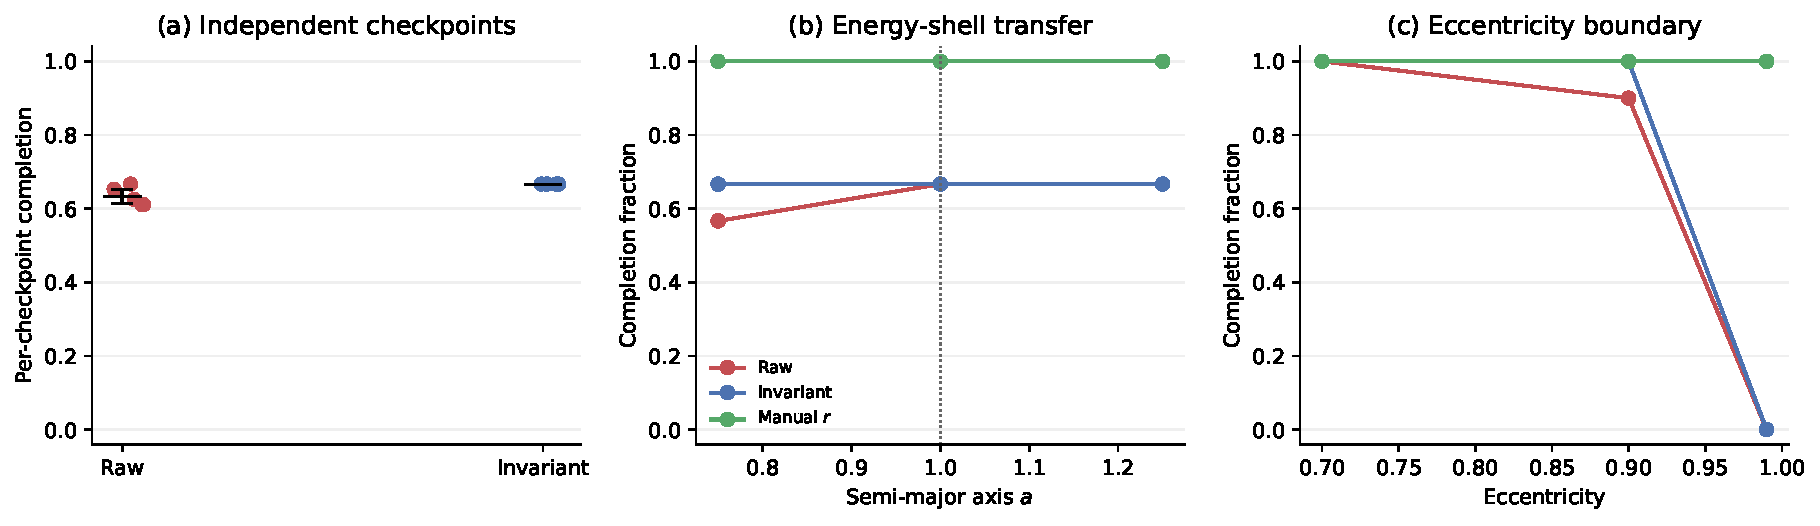
\includegraphics[width=\textwidth]{../fig_checkpoint_generalisation.pdf}
\caption{Completion of independently rollout-trained Kepler monitors under
the exact Hamiltonian and transformed step $h=0.04$.
(a) Each coloured point is one checkpoint evaluated on 72 scenarios;
black marks show the checkpoint mean and 95\% checkpoint-bootstrap
interval. Horizontal jitter separates points with equal completion.
(b) Fractions at each semi-major axis aggregate 120 evaluations per learned
architecture and 24 manual controls; the dotted line marks the training
value $a=1$.
(c) The corresponding eccentricity fractions have the same denominators.
Lines join the tested grid values and do not locate a continuous failure
threshold. Repeated scenarios share checkpoints; the invariant interval
collapses because the five observed completion fractions are equal.}
\label{fig:kepler-reliability}
\end{figure}
% Figure is an existing Matplotlib artifact from the independent-checkpoint
% analysis, visually checked against the saved raw/analysis records.
% The similarly named fig_monitor_generalisation belongs to earlier studies.

The failure region is concentrated at high eccentricity. At $e=0.7$,
both learned architectures complete all 120 evaluations. At $e=0.9$,
the raw architecture completes 108/120 and the invariant architecture
120/120. At $e=0.99$, neither architecture completes any of its 120
evaluations, whereas the manual control completes all 24 cases. Every
learning seed exhibits this high-eccentricity failure pattern. All 252
failed learned-monitor runs terminate at the fixed-point iteration limit;
their failure labels are not an energy-error threshold or a step-cap
censoring rule.

The remaining 12 raw failures occur at $a=0.75$, $e=0.9$. In that
$(a,e)$ cell, raw completion is 28/40, compared with 40/40 for the
invariant monitors. Both architectures complete every $e=0.9$ case at
$a=1$ and $a=1.25$, and both fail every $e=0.99$ case at all three
semi-major axes. The marginal fractions in Figure~\ref{fig:kepler-reliability}(b)
average over eccentricities; the joint $(a,e)$ pattern locates the
invariant-input improvement.

Checkpoint variability gives a complementary view. The five raw
checkpoints complete between 44 and 48 of their 72 scenarios, whereas
each invariant checkpoint completes 48/72. The matched-seed mean
invariant-minus-raw difference is 3.3 percentage points; the 95\%
checkpoint-bootstrap interval is 1.4--5.3 percentage points. This
interval describes seed variability on the fixed grid; a degenerate
invariant interval gives no certainty beyond it.

The symmetry comparison examines consistency as well as completion. Holding checkpoint, $a$, $e$ and initial anomaly fixed defines a
group of four rotation--momentum-direction variants. Invariant monitors
give the same completion status within all 90 such groups; raw monitors
do so in 83 of 90. Uniformity includes all-failure groups and establishes symmetry consistency,
not successful deployment.
The separate single-teacher distillation study also favours invariant
inputs in its fixed-point comparison. Its teacher dependence, training
objective and three-period horizon give it a supporting role; it cannot
count as an additional independent repetition of rollout training.
The next subsection examines its solver comparison.

Returned-endpoint residual replay preserves every completion status in
the 792-case baseline grid. The reliability pattern thus survives that
explicit check. We next examine periapsis diagnosis and solver interventions.

\subsection{Periapsis diagnostics and solver interventions}
\label{sec:periapsis-interventions}

The diagnostic study uses the ten frozen rollout-trained checkpoints and
manual $g=r$ to relate failures to periapsis profiles, then tests solver
and step interventions. Evaluating each
on 36 reference-orbit families gives 396 orbit records. Each family
diagnostic is shared by the two initial anomalies in the deployment grid;
the subsequent comparison with 792 rollout outcomes therefore does not
contain 792 independent diagnostic measurements.

Figure~\ref{fig:periapsis-mechanism} connects the saved monitor profiles,
reference diagnosis and failure projections to the Kepler scale
calculation. Table~\ref{tab:periapsis-diagnostic} summarises the $e=0.99$ orbits at
$h=0.04$. At periapsis, the median $g_\theta/r$ is 18.1 for raw monitors
and 8.87 for invariant monitors, compared with exactly one for $g=r$.
Every learned monitor on these orbit families has
$\rho_{\max}^{\mathrm{ref}}>1$, whereas the manual monitor remains below
one on all 36 families, with a maximum of 0.326. The invariant inputs
reduce variation in the periapsis monitor ratio on this grid, but do not
prevent the large values relative to the prescribed radial time scale.
These finite-radius observations establish neither an asymptotic law
as $r\to0$ nor loss-term causality. The ratio $g_\theta/r$ is not a
convergence criterion; the diagnostic uses the full Hessian
\eqref{eq:extended-hessian}.

\begin{table}[t]
\centering
\caption{Reference-orbit diagnostics for $e=0.99$ at $h=0.04$.
Entries are medians with the observed range in brackets. The sample
counts refer to checkpoint--orbit families, before duplication across
the two initial anomalies. The spectral radius is the sampled
reference-orbit maximum, not the iteration matrix at a computed endpoint.}
\label{tab:periapsis-diagnostic}
\begingroup
\renewcommand{\baselinestretch}{1}\small
\setlength{\tabcolsep}{4pt}
\begin{tabular}{lrrr}
\toprule
Monitor & Families & $g_\theta/r$ at periapsis &
 $\rho_{\max}^{\mathrm{ref}}$ \\
\midrule
Raw & 60 & 18.1 [4.13, 95.2] & 6.12 [1.43, 31.7] \\
Invariant & 60 & 8.87 [6.40, 14.8] & 3.31 [1.70, 7.54] \\
Manual $g=r$ & 12 & 1 [1, 1] & 0.283 [0.253, 0.326] \\
\bottomrule
\end{tabular}
\endgroup
\end{table}

The registered rule $\rho_{\max}^{\mathrm{ref}}\ge1$ identifies 240 of
the 252 failed rollouts and classifies all 540 completed rollouts as
complete. Thus its confusion matrix contains 240 true failures,
12 missed failures, zero false failures and 540 true completions:
accuracy is 98.5\% and failure sensitivity is 95.2\% on this grid.
All twelve misses are raw-monitor evaluations at $a=0.75$, $e=0.9$,
where the reference statistic remains below one. The procedure was
frozen before the full diagnostic calculation, but the rollout labels
were already known and development pilots had been run. The evidence is retrospective. The misses show that a sampled value
below one cannot certify completion. Prospective use is tested in the
later checkpoint study.

A separate accepted-iterate audit does not support an early conditioning
warning on its tested grid. Across 1056 recorded rollouts from the
distilled and independently trained studies, one observation per rollout
at each of accepted steps 10, 50 and 100 shows smaller median contraction
proxy and endpoint condition number, and larger median minimum singular
value, for eventual failures. At step 100, the median condition numbers
are 1.0096 for the 716 eventual completions and 1.0078 for the 340
eventual failures. Supplementary Material, Section S4.1, gives the scaled
operators, distributions and denominators. These contrasts describe pooled observations at
early accepted numerical midpoints. They validate no online classifier
and leave later loss of contraction possible.
$\rho_{\max}^{\mathrm{ref}}$, in comparison, samples a full reference orbit.

Positivity does not ensure completion; a low-validation-error counterexample
is reported in Section~\ref{sec:training-factorisation}.

Failure localisation provides a second, distinct check. Mapping each
recorded failure time to the analytic reference orbit places 250 of
252 failures below the training radius $r=0.1$. However, only 60 lie
within twice the periapsis radius; 231 lie within five times that radius.
The median reference radius divided by the periapsis radius is 2.70,
with a range of 1.00--8.20. Failures concentrate at small radii but extend beyond the immediate
periapsis neighbourhood. These locations project recorded times onto the reference orbit;
the failed iterates themselves were not located.

The shrinking Kepler time scale explains why a positive monitor can still
allocate inadequate resolution. With gravitational parameter one, the
local gravitational time scale is $t_{\mathrm{loc}}=r^{3/2}$. Freezing
the monitor at a state gives the physical step estimate $\Delta t\simeq
hg_\theta$ and the dimensionless resolution indicator
\begin{equation}
 \chi(r)=\frac{hg_\theta}{r^{3/2}}.
 \label{eq:kepler-resolution-scale}
\end{equation}
For fixed $h$ and an approximately constant monitor, $\chi$ grows as
$r^{-3/2}$; the manual choice $g=r$ reduces this growth to $r^{-1/2}$.
A radius decrease from 0.1 to 0.01 therefore multiplies these indicators
by approximately 31.6 and 3.16, respectively. These factors estimate the resolution scale;
they do not measure growth in $\rho_{\max}^{\mathrm{ref}}$. The full
endpoint Jacobian also contains the monitor derivatives in
\eqref{eq:extended-hessian}. The radial factor mitigates the resolution
mismatch without keeping $\chi$ uniformly bounded as $r\to0$.
This explains the motivation for the tested factorisation while retaining
its finite-radius, solver-dependent interpretation.

The separate distilled-monitor study isolates the effect of replacing
fixed-point iteration with damped Newton for the same checkpoints and
deployment scenarios. Raw-monitor completion increases from 30/60 to
34/60: four cases are restored and none are lost. Invariant-monitor
completion is 44/60 under both solvers, but the successful sets differ:
40 cases complete under both, four only under fixed-point iteration,
four only under Newton, and twelve under neither. The manual $g=r$
control completes all twelve cases with each solver. Newton therefore
provides a limited, non-monotone intervention in this study; unchanged
aggregate completion for invariant monitors does not mean unchanged
individual outcomes. The single teacher and three-period horizon also
preclude pooling these counts with the one-period rollout-trained grid.
The original architecture--solver comparison is retained in Supplementary
Material, Section S4.2, with the associated symmetry-error summaries.

For the latter grid, applying \eqref{eq:diagnostic-step-intervention}
to all 252 failed learned-monitor runs reduces the step in every case.
The median factor $h_{\mathrm{test}}/h$ is 0.136, with a range of
0.0158--0.929. With the step budget increased from $10^5$ to
$2\times10^6$, 150/252 runs (59.5\%) complete with verified endpoint
acceptance and 102 still fail the solver. The original update-stop count
was 151; the successor loses one raw-monitor case, confirmed by a separate
scalar replay. Table~\ref{tab:step-intervention} retains all failures and
separates the additional $e=0.9$ raw-monitor cases from the high
eccentricity cases. All twelve diagnostic misses complete under this
intervention. This tests step-and-budget sensitivity without isolating monitor
plateauing as the sole failure cause.

\begin{table}[t]
\centering
\caption{Prescribed step reduction on previously failed rollout-trained
evaluations. The original checkpoint and scenario are retained; the
smaller-step protocol also allows a larger step budget. Completion means
reaching the prescribed horizon with verified endpoint residual acceptance,
without an additional trajectory-accuracy gate.}
\label{tab:step-intervention}
\begingroup
\renewcommand{\baselinestretch}{1}\small
\begin{tabular}{lrrr}
\toprule
Monitor and eccentricity & Reruns & Complete & Solver failure \\
\midrule
Raw, $e=0.9$ & 12 & 12 & 0 \\
Raw, $e=0.99$ & 120 & 84 & 36 \\
Invariant, $e=0.99$ & 120 & 54 & 66 \\
\midrule
Total & 252 & 150 & 102 \\
\bottomrule
\end{tabular}
\endgroup
\end{table}

Restored completion comes with substantial work and accuracy penalties.
For the 150 verified completed reruns only, the geometric mean of the
paired final-state closure-error ratio to manual $g=r$ at $h=0.04$ is
408. The field-call ratio is 17.7 when acceptance verification is included
in the numerator; its manual denominator retains the original stopping
rule, so it is not a comparison under identical verification overhead.
Each ratio pairs a scenario conditional on intervention
completion. The summaries are neither ratios of aggregate means nor
summaries of all 252 attempts. Field-call counts also exclude reference-diagnostic cost and
do not equate automatic-differentiation and analytic-gradient arithmetic.
Cross-environment wall-time ratios are not used for this comparison.
The observational replay found 135 returned solves above $10^{-12}$ under
the original update stop, with maximum residual $4.46\times10^{-11}$.
The verified successor accepts none above tolerance. Its completed reruns
therefore provide evidence of execution recovery
without comparable trajectory accuracy under the tested protocol.

Further refinement and alternative solvers remain open. We next examine
training-domain coverage and monitor parameterisation.

\begin{figure}[p]
\centering
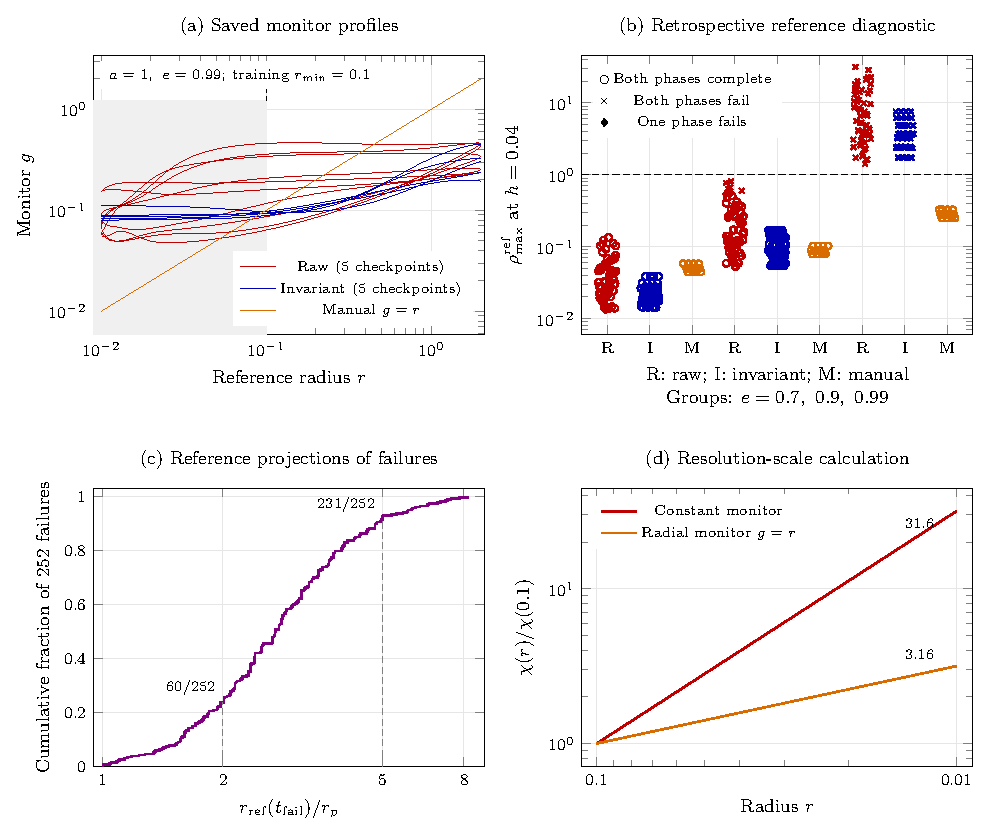
\includegraphics[width=\textwidth]{fig_periapsis_new.pdf}
\begingroup
\renewcommand{\baselinestretch}{1}\small
\caption{Kepler monitor behaviour and reference diagnostics.
(a) Saved profiles on the $a=1$, $e=0.99$ orbit, with orientation zero
and forward momentum: five checkpoints per learned architecture and
one manual control. Inbound and outbound legs are drawn separately;
shading marks radii below the training minimum 0.1.
(b) Retrospective comparison at $h=0.04$: each of the 396 points is
one checkpoint--orbit family, with symbols encoding the outcomes of
its two initial anomalies. Colour distinguishes monitor architecture;
the dashed line is the reference threshold one.
(c) Analytic reference radii at the recorded clocks of 252 failures,
normalised by periapsis radius $r_p$; these are not failed-iterate radii.
(d) Normalised $\chi$ from \eqref{eq:kepler-resolution-scale} for
constant and radial monitors. This panel is a scale calculation,
not a fit to the measured spectral radius.}
\label{fig:periapsis-mechanism}
\endgroup
\end{figure}
\subsection{Training-domain changes and Sundman factorisation}
\label{sec:training-factorisation}

We compare three newly trained invariant-feature arms:
an unfactored monitor trained at $e=0.99$, and the factored monitor
\eqref{eq:factored-monitor} trained at either $e=0.9$ or $e=0.99$.
Figure~\ref{fig:factorisation-study} summarises the resulting completion,
monitor scale, reference diagnostic and completed-run accuracy--work
comparison. All use $a=1$, five matched seed identities and the same one-period
deployment grid as the baseline. The new study contains 15 checkpoints,
540 checkpoint--orbit diagnostics and 1080 rollouts. Deployment retains
$h=0.04$ and the original fixed-point protocol. The smaller steps and
larger budget of Section~\ref{sec:periapsis-interventions} are not used.

\begin{table}[t]
\centering
\caption{Completion after changing the training orbit and monitor recipe.
Each learned row contains five checkpoints and 360 deployment evaluations,
with 120 at each deployment eccentricity. The baseline row is the frozen
invariant-monitor comparison from Section~\ref{sec:kepler-reliability}.
Training eccentricity refers to the $a=1$ training orbit. Completion is
reported separately from trajectory accuracy.}
\label{tab:training-factorisation}
\begingroup
\renewcommand{\baselinestretch}{1}\small
\setlength{\tabcolsep}{4pt}
\begin{tabular}{lrrrrr}
\toprule
 & Training & \multicolumn{3}{c}{Deployment eccentricity} & \\
\cmidrule(lr){3-5}
Monitor & $e$ & 0.7 & 0.9 & 0.99 & Total \\
\midrule
Unfactored, baseline & 0.9 & 120/120 & 120/120 & 0/120 & 240/360 \\
Unfactored, new & 0.99 & 120/120 & 120/120 & 0/120 & 240/360 \\
Factored, new & 0.9 & 120/120 & 120/120 & 120/120 & 360/360 \\
Factored, new & 0.99 & 120/120 & 120/120 & 120/120 & 360/360 \\
\bottomrule
\end{tabular}
\endgroup
\end{table}

Moving the unfactored monitor's training eccentricity from 0.9 to 0.99
reduces the training periapsis from 0.1 to 0.01. Nevertheless, the new
unfactored arm completes 240/360 evaluations and fails all 120 at
$e=0.99$, reproducing the baseline completion pattern
(Table~\ref{tab:training-factorisation}). Each checkpoint completes
48/72 scenarios. Its high-eccentricity reference diagnostics also remain
above the threshold: the median $\rho_{\max}^{\mathrm{ref}}$ is 5.49,
with a range of 2.58--14.2, and the median periapsis $g_\theta/r$ is 13.9,
with a range of 7.86--42.5. The added radial coverage leaves the observed boundary
unchanged for this recipe. Coverage remains incomplete: the smallest
deployment periapsis, 0.0075, lies below the new training minimum, and
one training orbit does not cover the different energy shells. Complete
phase-space coverage has therefore not been tested.

Training fit further limits the interpretation of this negative result.
The five selected validation state MSEs for the new unfactored arm range
from $2.57\times10^{-8}$ to 6.60, with median 1.01. Four checkpoints thus
have much larger validation errors than the best-fitting checkpoint;
the arm does not demonstrate uniformly successful optimisation on the
changed training orbit. However, even the checkpoint with validation MSE
$2.57\times10^{-8}$ fails all 24 of its $e=0.99$ deployments. Low error
in the validation computation is therefore not sufficient here to ensure
completion under the deployed solver. Validation uses the unrolled
training calculation described in Section~\ref{sec:monitor-training},
whose finite iteration count and horizon differ from deployment.
Neither the failed arm nor this single checkpoint establishes that
training on a sufficiently sampled deployment domain could never work.

Both factored arms complete all 360 evaluations, including all 120
high-eccentricity cases per arm. Every checkpoint completes 72/72
scenarios, giving a paired increase of 24/72, or 33.3 percentage points,
relative to its matched baseline invariant checkpoint. At $e=0.99$ the
increase is 24/24 for each seed. The identical completion contrasts make
the saved checkpoint-bootstrap intervals degenerate; they do not remove
uncertainty beyond these five seeds and the fixed grid. In particular,
the arm trained at $e=0.9$ completes despite retaining the original
training-radius minimum of 0.1. Within this comparison, extending the
training orbit to $e=0.99$ is not required for completion by the tested
factored recipe.

The new endpoint review preserves every completion status and accepted-step
count in all 1080 evaluations under verified acceptance. Observation at the
original stopping rule finds 20 returned solves above $10^{-12}$ in the
expanded unfactored arm, but none in either factored arm. The factored
arms' maximum returned residuals are $6.63\times10^{-13}$ and
$5.20\times10^{-13}$, respectively. The checks cover a finite grid and include
terminal-search candidates. They provide no convergence theorem.

The reference diagnostics agree with this change in outcome. On
$e=0.99$ families, the factored arms trained at $e=0.9$ and $e=0.99$
have median periapsis $g_\theta/r$ of 1.12 and 0.836, respectively.
Their corresponding median $\rho_{\max}^{\mathrm{ref}}$ values are
0.309 and 0.212; the largest values over all deployment families are
0.479 and 0.307. For these arms, the output constraint
$0<g_\theta<2r$ prevents a positive monitor plateau as $r\to0$ in
exact arithmetic. It does not impose a positive uniform lower bound
on $g_\theta/r$ independent of the learned parameters, control monitor
derivatives, or establish convergence
of the implicit endpoint solver. The diagnostics and completed rollouts
are additional empirical evidence, distinct from that output bound.

For every newly trained checkpoint, the saved full reference diagnostic
finishes before that checkpoint's deployment evaluations begin. Applying
the previously registered threshold of one gives 120 true failures,
960 true completions, zero missed failures and zero false failures across
the 1080 new evaluations. All failures occur in the unfactored
high-eccentricity stratum. This is prospective use on new checkpoints,
but on a grid and with interventions informed by the earlier studies
and disclosed pilots. Two initial anomalies still share each family
diagnostic, and the two factored arms supply no failures with which to
estimate failure sensitivity within those arms. Complete agreement supports the diagnostic within
this designed evaluation. It guarantees neither distribution-free
prediction nor global stability.

The initialisation and training differences specified in
Sections~\ref{sec:monitor-training} and \ref{sec:benchmark-design}
remain material to attribution. The factored arms have validation-MSE medians
of $1.15\times10^{-5}$ and $1.44\times10^{-3}$ on their respective
training orbits, but these are not a common validation domain. Four
epochs are skipped for non-finite loss or gradient norm in one
$e=0.99$ factored training run; none are skipped in the other arms.
Accordingly, these results assess the complete recipes and do not isolate
factorisation from initialisation or optimisation effects.

Manual $g=r$ already completes the grid. The next comparison assesses
accuracy and work.

% TODO(author): B1. A loss ablation is needed to identify a cause of plateauing.
\begin{figure}[p]
\centering
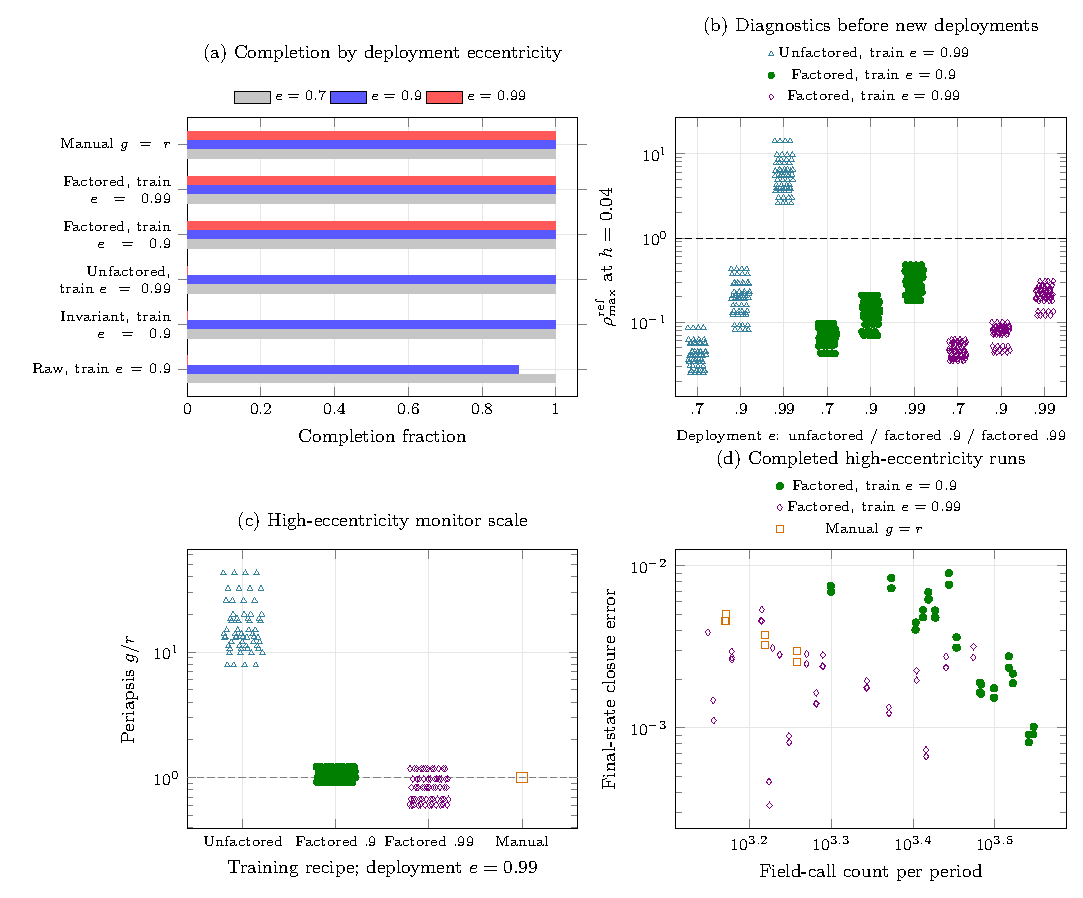
\includegraphics[width=\textwidth]{fig_factorisation_new.pdf}
\begingroup
\renewcommand{\baselinestretch}{1}\small
\caption{Training-domain changes and Sundman-factored recipes at
$h=0.04$. (a) Completion fractions: each eccentricity contains
120 evaluations per learned arm and 24 manual controls.
(b) Reference diagnostics finished before deployment of the 15 new
checkpoints; 540 family points each serve two rollout phases.
(c) Periapsis $g/r$ on $e=0.99$ families: 60 points per new arm;
the manual value is exactly one.
(d) Field calls and closure error for all completed $e=0.99$ runs:
120 per factored arm and 24 manual controls. The expanded-domain
unfactored arm contributes no points because all 120 runs fail.
These are common-step comparisons of complete recipes with differing
initialisation and training settings, rather than an isolated
factorisation effect or a matched-cost comparison.}
\label{fig:factorisation-study}
\endgroup
\end{figure}
\subsection{Accuracy--cost trade-offs and scope tests}
\label{sec:cost-scope}

The historical cost sweep contains the ten baseline unfactored monitors;
the newly trained factored arms receive a separate common-step comparison.

Figure~\ref{fig:accuracy-cost} shows the 38-configuration Kepler sweep
on 18 scenarios. Raw monitors complete 60/90 evaluations at each of
the three transformed steps, 0.08, 0.04 and 0.02.
Invariant-monitor completion is 60/90
at the two larger steps and 61/90 at $h=0.02$. The one additional
completion occurs at $e=0.99$; it leaves every learned configuration
short of completing all 18 scenarios. Direct physical-time midpoint
completes 10/18, 12/18 and 12/18 cases at physical steps 0.02, 0.01 and
0.005, respectively. Both adaptive midpoint tolerances and all three
manual Sundman steps complete 18/18. The returned-endpoint residual
replay preserves every completion-versus-failure classification in this
684-run sweep. The figure nevertheless uses the original registered
counts and timings; replay adds verification work and is a separate
execution record.

\begin{figure}[t]
\centering
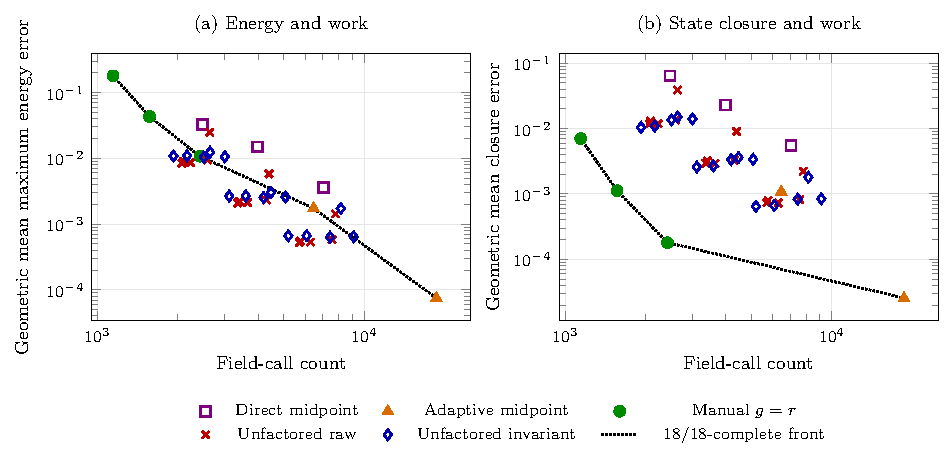
\includegraphics[width=\textwidth]{fig_accuracy_cost_new.pdf}
\begingroup
\renewcommand{\baselinestretch}{1}\small
\caption{Accuracy and work on the Kepler cost grid. Each point is one
configuration, aggregated by geometric means over its completed runs.
There are 38 configurations and 18 registered scenarios per configuration.
Filled manual and adaptive markers represent 18/18 completion; direct
midpoint squares, learned invariant diamonds and learned raw crosses
represent incomplete configurations. Their error summaries use different
completed subsets and cannot be read as comparisons at equal reliability.
Dotted lines connect the non-dominated 18/18-complete configurations only;
they do not represent an interpolated optimum. Work uses the original
field-call accounting, including adaptive rejected trials and endpoint
alignment; different gradient implementations need not have equal
arithmetic cost. Training and reference-diagnostic costs are excluded.
The newly trained factored arms are absent from this sweep.}
\label{fig:accuracy-cost}
\endgroup
\end{figure}

Among configurations that complete the common grid, the energy--field-call
front contains the three manual Sundman steps and both adaptive
tolerances. The closure--field-call front contains the three manual steps
and adaptive midpoint at relative tolerance $10^{-7}$. The closure--wall-time
front contains the two adaptive configurations on the recorded host.
Thus no baseline learned configuration qualifies for a full-grid front.
Smaller learned steps improve errors on many completed cases, but their
conditional error points do not establish full-grid superiority.
The fronts rank only the registered configurations under their solver
and work-accounting protocols. The supplementary record retains configuration peak
resident memory, measured for a fresh process across 18 scenarios.
This measurement does not isolate per-rollout allocation.
Supplementary Material, Section S5.3, displays all 38 configuration-level
measurements, including incomplete configurations.

Figure~\ref{fig:factorisation-study}(d) displays the corresponding
high-eccentricity state-error and work measurements.
For the factored arms, the available comparison is instead at the common
step $h=0.04$, against manual $g=r$ on matching scenarios
(Table~\ref{tab:factored-cost}). Across all 360 evaluations, the arm
trained at $e=0.9$ has a geometric mean closure-error ratio of 2.42 and
field-call ratio of 1.77. For the arm trained at $e=0.99$, the ratios are
0.975 and 1.24. In the $e=0.99$ deployment stratum alone, the latter
arm's closure-error ratio is 0.500, while its field-call ratio is 1.22.
The error improvement in that stratum therefore comes with additional
field calls at this step; it is not a comparison at matched cost.
All ratios are geometric means of individual matched-scenario ratios,
with all factored evaluations completed. Their common manual denominators
are reused across checkpoints, so the 360 ratios are dependent and are
not 360 independent estimates of an efficiency gain. Cross-environment
wall-time ratios are excluded, and neither these ratios nor the original
fronts estimate the cost of training and deployment together.

\begin{table}[t]
\centering
\caption{Factored-monitor ratios to manual $g=r$ at the same transformed
step $h=0.04$. Values are geometric means of paired ratios; a value below
one means smaller error or fewer field calls in that aggregate.
``All'' denotes the full deployment grid. Every numerator run completes;
no claim of matched-cost advantage is made.}
\label{tab:factored-cost}
\begingroup
\renewcommand{\baselinestretch}{1}\small
\setlength{\tabcolsep}{4pt}
\begin{tabular}{llrrrr}
\toprule
Training $e$ & Deployment & Pairs & $E_{\mathrm{cl}}$ ratio & $E_H$ ratio & Field ratio \\
\midrule
0.9 & All & 360 & 2.42 & 0.899 & 1.77 \\
0.9 & $e=0.99$ & 120 & 0.863 & 1.14 & 1.73 \\
0.99 & All & 360 & 0.975 & 0.656 & 1.24 \\
0.99 & $e=0.99$ & 120 & 0.500 & 0.693 & 1.22 \\
\bottomrule
\end{tabular}
\endgroup
\end{table}

The learned-Hamiltonian entry study supplies a separate limitation.
None of its five trained candidates passes the predeclared fidelity
gate in Section~\ref{sec:controls-validation}. Held-out gradient
normalised RMSE ranges from 0.254 to 0.313 overall, against the threshold
0.01, and from 0.284 to 0.350 at $e=0.99$, against the stratum threshold
0.02. Since at least three accepted candidates are required, subsequent
monitor training and the planned solver comparison are not run; the
deployment artifact contains zero evaluations. The rejection is specific to this recipe and held-out states.
Section~\ref{sec:continuous-equivalence} explains why monitor learning
cannot replace Hamiltonian verification; it gives no nonzero error lower
bound for rejected candidates.

Finally, both non-Kepler benchmarks complete all their registered
evaluations. The learned monitors account for 144 modal and 72 Duffing
runs; prescribed-monitor midpoint and resolved Verlet add 72 control
runs, giving 288 in total. With three checkpoints per input architecture,
these results establish completion on the tested energy labels, initial
conditions and momentum directions. They do not establish broad
reliability across large coupled Hamiltonian systems: the modal benchmark
has 32 state variables, is separable in modal coordinates, and tests only
frequency ratios 10 and 20; Duffing has two state variables.

Table~\ref{tab:cross-system-accuracy} retains energy and state error
alongside work. Both learned architectures have smaller median maximum
state error than the prescribed monitor at these settings, with higher
median field-call counts. The modal learned trajectories illustrate why
small energy variation is insufficient evidence of state accuracy:
median maximum energy errors are about $6\times10^{-5}$, while median
maximum state discrepancies are about 0.22. Each system's coordinates and horizon define its state metrics.
The table compares registered settings; it does not define a cost front.

\begin{table}[t]
\centering
\caption{Non-Kepler accuracy and work at the registered deployment
settings. Counts include all completed evaluations in each row; other
entries are medians. $E_H$ is maximum absolute energy variation, and
state error is the maximum sampled Euclidean discrepancy from the
original Verlet reference at step 0.001. Field calls measure work rather
than equal arithmetic operations. The Verlet control is not assigned
zero true state error; its reference uncertainty is assessed separately.}
\label{tab:cross-system-accuracy}
\begingroup
\renewcommand{\baselinestretch}{1}\small
\setlength{\tabcolsep}{5pt}
\begin{tabular}{lrrrr}
\toprule
Monitor & Evaluations & $E_H$ & Max. state error & Field calls \\
\midrule
\multicolumn{5}{l}{Modal benchmark, $T=10\pi$} \\
Raw & 72 & $5.99\times10^{-5}$ & 0.224 & 50\,404 \\
Reversal-even & 72 & $5.52\times10^{-5}$ & 0.229 & 49\,860.5 \\
Prescribed & 24 & $3.34\times10^{-5}$ & 0.557 & 34\,845 \\
\midrule
\multicolumn{5}{l}{Duffing benchmark, $T=20$} \\
Raw & 36 & $3.75\times10^{-5}$ & 0.00201 & 8\,911 \\
Reversal-even & 36 & $1.05\times10^{-4}$ & 0.00491 & 8\,111.5 \\
Prescribed & 12 & $1.64\times10^{-4}$ & 0.0229 & 4\,428 \\
\bottomrule
\end{tabular}
\endgroup
\end{table}

Reference refinement over all 36 non-Kepler scenarios gives median
observed orders for maximum state discrepancy of 2.000 in both systems.
Propagating the saved Richardson reference-error estimates into the
reported median state errors retains separation between learned and
prescribed monitors. However, the modal raw and reversal-even final-state
error intervals overlap, so their final-error ordering is unresolved
under that sensitivity calculation. Estimated reference error determines these
intervals; they are neither rigorous bounds nor sampling confidence
intervals. Positive estimated uncertainty also remains for the finest
reference, which cannot serve as an exact zero-error comparator. The scope tests therefore add finite
examples of successful execution with measurable accuracy--work
trade-offs; they do not extend the Kepler reference-orbit threshold to
an untested general system.

% TODO(author): B2. Cost-matched factored-monitor comparisons remain untested.
% TODO(author): B3. Larger non-collapsing stiff systems require new experiments.
% TODO(author): B4. Learned-H deployment requires candidates passing the gate.

\section{Discussion}
\label{sec:discussion}
\subsection{Implications for monitor design}
\label{sec:design-implications}

Both tested Kepler recipes restore completion with
$g_\theta=2r\sigma(f_\theta(\phi))$, which embeds a classical time scale.
The indicator $\chi=hg_\theta/r^{3/2}$ illustrates the reduced resolution
mismatch near periapsis, without supplying a universal scale for other
stiffness mechanisms or controlling monitor derivatives. Symmetry
constraints improve consistency but do not rescue the baseline
highest-eccentricity cases. Positivity and small validation error are also
insufficient completion criteria. The energy-variance and inverse-monitor
losses remain surrogates whose individual effects require ablation.

Validation should assess Hamiltonian fidelity separately from the
monitor--solver combination, then test endpoint acceptance, state accuracy
and resource use at the intended step. Reference diagnostics can inform
interventions where an analytic orbit is available. Manual $g=r$ already
completes the grid, so a learned correction needs an accuracy--work
comparison to establish value beyond usability. The modal tests reinforce
the need to measure state error alongside invariant variation.

\subsection{Limits of the evidence and unresolved questions}
\label{sec:evidence-limits}

Continuous equivalence requires a positive monitor and an exact
zero-energy flow; the energy bound also requires compact confinement away
from singularities. The closed convex self-map and uniform norm conditions
in \eqref{eq:banach-sufficient-condition} remain unverified along entire
numerical trajectories, so no global discrete theorem or necessary radial
decay rate follows. Returned-residual checks cover the intervention and
new training arms, but observational and residual-enforced replay disagree
on one completion. The terminal search sets the reported clock to the
horizon while retaining the last candidate state. The largest absolute
clock-increment discrepancy over completed replay cases,
$7.36\times10^{-14}$, checks terminal matching only. Zero recorded time
error is not an independent clock-accuracy measurement; accumulated clock
and trajectory accuracy remain outside this check. Exact fixed-step
midpoint symplecticity does not automatically extend to finite solves or
the state-dependent terminal procedure.

Reference diagnostics require full-orbit Hessian work and separate online
validation. Sampling, reference departure, non-normality and nonlinear
basin effects limit interpretation. Failure-radius projections use
recorded times, not failed iterates. The pooled early accepted-iterate
contrasts do not support the proposed warning, and matched step indices
do not match physical times or orbital phases. Statistical replication
comprises five checkpoints per Kepler arm and three per non-Kepler input
architecture on dependent grids: two initial anomalies share each family
diagnostic, and distilled students share a teacher. Bootstrap intervals
describe training variation on these grids, even when degenerate; they
give no certainty elsewhere. Baseline labels are known, while new-checkpoint
diagnostics are prospective within the informed design. Complete agreement
supplies no population probability guarantee.

Factorisation changes together with output bias, state generation,
validation and non-finite handling, leaving isolated causality unresolved.
Expanded training misses part of the deployment domain and is not
uniformly well optimised; finite unrolling and detached clocks also differ
from deployment. Causal attribution needs controlled initialisation, loss
and broader-domain training studies. Efficiency is likewise unresolved:
factored arms use a common step, survivor summaries exclude failures, and
field calls carry unequal arithmetic costs. Training and reference
diagnostics are excluded from the reported comparisons, while step recovery
enlarges the budget. Practical advantage requires matched-work or
matched-error comparisons with the relevant overhead included.

The evidence remains primarily finite-radius exact-H Kepler. No learned-H
candidate passes the gate, and modal/Duffing checks cover limited
dimensions, frequency ratios and horizons. Richardson uncertainties are
estimates. Larger coupled systems and other stiffness mechanisms need
new evidence.

\section{Conclusions}
\label{sec:conclusions}

On the exact zero-energy surface, a positive time monitor preserves the
supplied physical-time flow, but its derivatives affect finite endpoint
solving. On the tested exact-H Kepler grid, positivity and low validation
error do not ensure completion; reference diagnostics and solver
interventions expose this gap. Both recipes learning a bounded correction
to $g=r$ complete their grids with fresh returned-residual verification.
These complete-recipe comparisons support encoding a known time scale.

Isolated factorisation causality and matched-cost advantage remain
unresolved; manual $g=r$ already completes the same scenarios. Deployment
evaluation should report whether runs finish, their state accuracy and
invariant variation, and the work they require. Online diagnostics,
accepted-fidelity learned-H deployment and larger coupled systems
remain open.

\section*{Code and data availability}
The local reproducibility package holds the implementation, trained
checkpoints and registered numerical records. They have not yet been
deposited in a public repository or persistent data archive.
\texttt{src/models/pasnet.py} defines the PASNet model and implicit-midpoint
rollout; the corresponding \texttt{experiments/}
and \texttt{results/} directories contain experiment drivers, validation
records and configuration manifests. Validation scripts accompany
these files in the local package. The public repository link, archive
citation, persistent identifier and approved code/data licences remain
to be finalised.



\section*{Declaration of competing interest}
The authors declare that they have no known competing financial interests
or personal relationships that could have appeared to influence the work
reported in this paper.

% Author identities, affiliations and corresponding email are supplied.
% Funding and competing interests confirmed; no acknowledgments requested.
% TODO(author): Complete CRediT using SUBMISSION_METADATA_TEMPLATE.md.
% TODO(author): Insert the accurate generative-AI preparation disclosure before
% References after the authors actually review and approve the stated content.

% Verified, selected references for the introduction; not an exhaustive survey.
% Embedded bibliography keeps this manuscript self-contained for the editor.
\begin{thebibliography}{99}
\bibitem{Hairer2006}
E. Hairer, C. Lubich, G. Wanner,
\emph{Geometric Numerical Integration: Structure-Preserving Algorithms
for Ordinary Differential Equations}, 2nd ed., Springer, Berlin, 2006.
\href{https://doi.org/10.1007/3-540-30666-8}{doi:10.1007/3-540-30666-8}.

\bibitem{Sundman1913}
K.~F.~Sundman,
``M\'emoire sur le probl\`eme des trois corps,''
\emph{Acta Mathematica} 36 (1913) 105--179.
\href{https://doi.org/10.1007/BF02422379}{doi:10.1007/BF02422379}.

\bibitem{Preto1999}
M. Preto, S. Tremaine,
A class of symplectic integrators with adaptive time step for separable
Hamiltonian systems,
The Astronomical Journal 118 (1999) 2532--2541.
\href{https://doi.org/10.1086/301102}{doi:10.1086/301102}.

\bibitem{Blanes2012}
S. Blanes, A. Iserles,
Explicit adaptive symplectic integrators for solving Hamiltonian systems,
Celestial Mechanics and Dynamical Astronomy 114 (2012) 297--317.
\href{https://doi.org/10.1007/s10569-012-9441-z}{doi:10.1007/s10569-012-9441-z}.

\bibitem{Duruisseaux2021}
V. Duruisseaux, J. Schmitt, M. Leok,
Adaptive Hamiltonian variational integrators and applications to symplectic
accelerated optimization,
SIAM Journal on Scientific Computing 43 (2021) A2949--A2980.
\href{https://doi.org/10.1137/20M1383835}{doi:10.1137/20M1383835}.

\bibitem{Ye2025}
K. Ye, Z. Cai, M. Wang, K. Yang, X. Liu,
An adaptive symplectic integrator for gravitational dynamics,
Astronomy \& Astrophysics 699 (2025) A170.
\href{https://doi.org/10.1051/0004-6361/202451822}{doi:10.1051/0004-6361/202451822}.

\bibitem{Knauf2025}
A. Knauf, Regularisation by Hamiltonian extension,
Nonlinearity 38 (2025) 075033.
\href{https://doi.org/10.1088/1361-6544/adf0d8}{doi:10.1088/1361-6544/adf0d8}.

\bibitem{Reich1999}
S. Reich, Backward error analysis for numerical integrators,
SIAM Journal on Numerical Analysis 36 (1999) 1549--1570.
\href{https://doi.org/10.1137/S0036142997329797}{doi:10.1137/S0036142997329797}.

\bibitem{Greydanus2019}
S. Greydanus, M. Dzamba, J. Yosinski,
Hamiltonian neural networks,
Advances in Neural Information Processing Systems 32 (2019).
\href{https://proceedings.neurips.cc/paper/2019/hash/26cd8ecadce0d4efd6cc8a8725cbd1f8-Abstract.html}{NeurIPS proceedings}.

\bibitem{Jin2020}
P. Jin, Z. Zhang, A. Zhu, Y. Tang, G. E. Karniadakis,
SympNets: Intrinsic structure-preserving symplectic networks for identifying
Hamiltonian systems,
Neural Networks 132 (2020) 166--179.
\href{https://doi.org/10.1016/j.neunet.2020.08.017}{doi:10.1016/j.neunet.2020.08.017}.

\bibitem{Canizares2024}
P. Canizares, D. Murari, C.-B. Sch\"onlieb, F. Sherry, Z. Shumaylov,
Symplectic neural flows for modeling and discovery,
arXiv preprint (2024), revised 2026.
\href{https://arxiv.org/abs/2412.16787}{arXiv:2412.16787}.

\bibitem{Offen2022}
C. Offen, S. Ober-Bl\"obaum,
Symplectic integration of learned Hamiltonian systems,
Chaos 32 (2022) 013122.
\href{https://doi.org/10.1063/5.0065913}{doi:10.1063/5.0065913}.

\bibitem{David2023}
M. David, F. M\'ehats,
Symplectic learning for Hamiltonian neural networks,
Journal of Computational Physics 494 (2023) 112495.
\href{https://doi.org/10.1016/j.jcp.2023.112495}{doi:10.1016/j.jcp.2023.112495}.

\bibitem{Thapar2026}
V. Thapar, A. Gupta,
Machine learning Hamiltonian dynamical systems with sparse and noisy data,
arXiv preprint arXiv:2604.17470 (2026).
\href{https://arxiv.org/abs/2604.17470}{arXiv:2604.17470}.

\bibitem{Janik2025}
K. Janik, P. Benner,
Time-adaptive SympNets for separable Hamiltonian systems,
arXiv preprint (2025).
\href{https://arxiv.org/abs/2509.16026}{arXiv:2509.16026}.

\bibitem{Janik2026}
K. Janik, P. Benner,
Time-Adaptive H\'enonNets for Separable Hamiltonian Systems,
Proceedings in Applied Mathematics and Mechanics 26 (2026) e70133.
\href{https://doi.org/10.1002/pamm.70133}{doi:10.1002/pamm.70133}.

\bibitem{Mou2026}
C. Mou, D. Xu, X. Zuo, K. Liu, Y. Zhang,
ATLAS-NN: Adaptive Transfer Learnable Symplectic-aware Neural Network
for Long-Time Hamiltonian Dynamics,
arXiv preprint (2026).
\href{https://arxiv.org/abs/2606.04447}{arXiv:2606.04447}.

\bibitem{Tao2016}
M. Tao, Explicit symplectic approximation of nonseparable Hamiltonians:
Algorithm and long time performance,
Physical Review E 94 (2016) 043303.
\href{https://doi.org/10.1103/PhysRevE.94.043303}{doi:10.1103/PhysRevE.94.043303}.

\bibitem{Mou2025PAS}
C. Mou, Y. Zhang, X. Zhu, Q. Zhuang,
PAS-Net: Physics-informed Adaptive Scale Deep Operator Network,
arXiv preprint (2025).
\href{https://arxiv.org/abs/2511.14925}{arXiv:2511.14925}.
\end{thebibliography}

\end{document}
